%\documentclass[11pt]{beamer}
\documentclass{beamer}
\usetheme{Amsterdam}
\usepackage[utf8]{inputenc}
\usepackage{amsmath}
\usepackage{amsfonts}
\usepackage{amssymb}
\usepackage{hyperref}
\author{Callerisa \and Fontany-Legall \and Qui}
\title{Modélisation d'une colonie de fourmis}
%\setbeamercovered{transparent} 
%\setbeamertemplate{navigation symbols}{} 
%\logo{} 
\institute{Université de Nice} 
\date{\today} 
%\subject{} 
\begin{document}

\begin{frame}

\titlepage
\end{frame}

\begin{frame}
\tableofcontents
\end{frame}


\section{Introduction}
\subsection{Contexte}
\subsection{Etat de l'art}
\begin{frame}
\frametitle{}
\framesubtitle{Contexte et état de l'art}
\begin{block}{Contexte}
\begin{itemize}
\item Problème du voyageur de commerce
\end{itemize}
\end{block}

\begin{block}{État de l'art}
\begin{itemize}
\item routage réseau
\item conception de circuits nanoélectroniques
\item traitement d'images
\item Etc.
\end{itemize}
\end{block}
\end{frame}

\subsection{Question Scientifiques}
\begin{frame}
\frametitle{Introduction}
\framesubtitle{Question Scientifiques}
\begin{itemize}
\item La présence de chercheuses a-t-elle une réelle influence sur l'efficacité de la récolte ?
\item Si oui, quelle est cette influence ?
\item Comment évolue-t-elle en fonction de le proportion de chercheuses ? 
\end{itemize}
\end{frame}

\section{Modélisation}
\subsection{Hypothèse simplificatrices}
\begin{frame}
\frametitle{Modélisation}
\framesubtitle{}
\begin{block}{Hypothèse simplificatrices}
\begin{itemize}
\item Les fourmis retrouvent le chemin vers le nid au flair.
\item Le mouvement des fourmis qui ne suivent pas de phéromones
est aléatoire.
\item Les conditions environnementales sont constantes
\item Uniquement deux types de fourmis : ramasseuses / chercheuses
\end{itemize}
\end{block}
\end{frame}

\subsection{Description du modèle}
\begin{frame}
\frametitle{Modélisation}
\framesubtitle{}
\begin{block}{Description du modèle}
\begin{itemize}
\item Ajout d'un nouveau type de fourmis
\item Paramétrage du pourcentage de chaque type de fourmi
\item Paramétrage de la nourriture
\end{itemize}
\end{block}
\end{frame}


\begin{frame}
\frametitle{Modélisation}
\begin{figure}
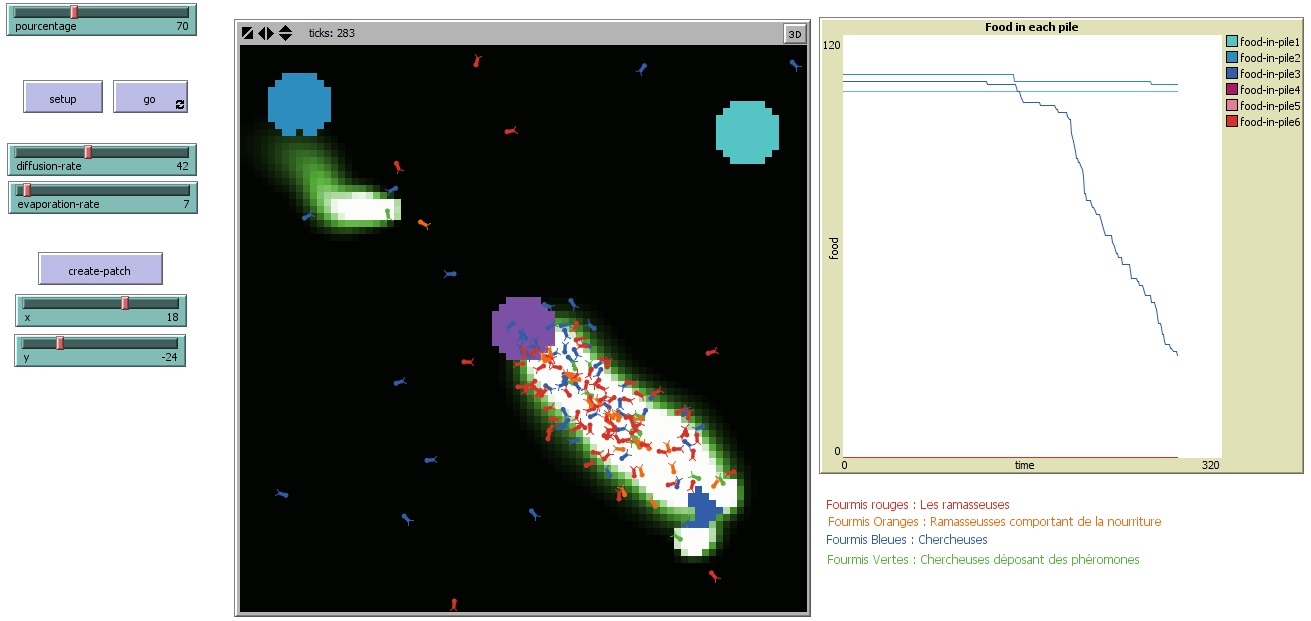
\includegraphics[scale=0.3]{Modelisation.jpg}
\caption{Interface de la simulation}
\end{figure}
\end{frame}

\section{Simulation}
\subsection{Cadre expérimental}
\begin{frame}
\frametitle{Simulation}
\framesubtitle{}

\begin{block}{Cadre expérimental}
\begin{itemize}
\item Netlogo 5.0.1
\item Modèle du MIT étendu
\end{itemize}
\end{block}
\end{frame}


\subsection{Protocole}
\begin{frame}
\frametitle{Simulation}
\begin{block}{Protocole}
\begin{itemize}
\item Utilisation de BehaviorSpace
\item Variation du pourcentage de chercheuses dans [1;90] par pas de 5 (18 runs)
\item Répéter pour différentes distances des tas de nourriture
\item Noter la durée de chaque simulation
\item Moyenne des trois fichiers produits
\item Régression polynomiale dans R pour trouver une relation
\end{itemize}
\end{block}
\end{frame}

\section{Résultats}
\begin{frame}
\frametitle{Résultats}
\begin{figure}
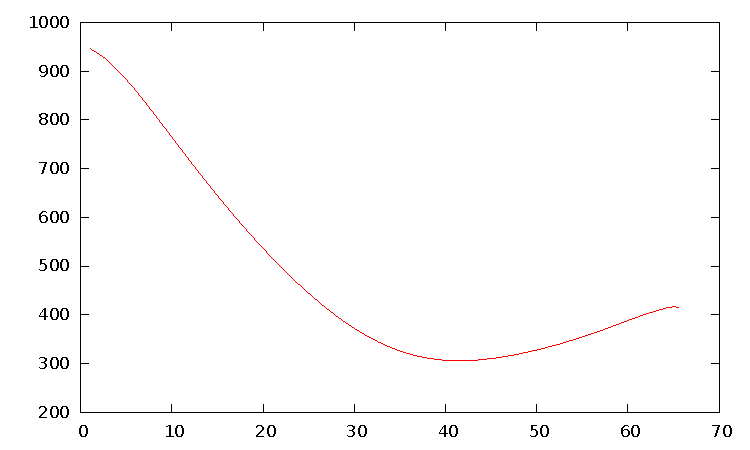
\includegraphics[scale=0.3]{near.pdf}
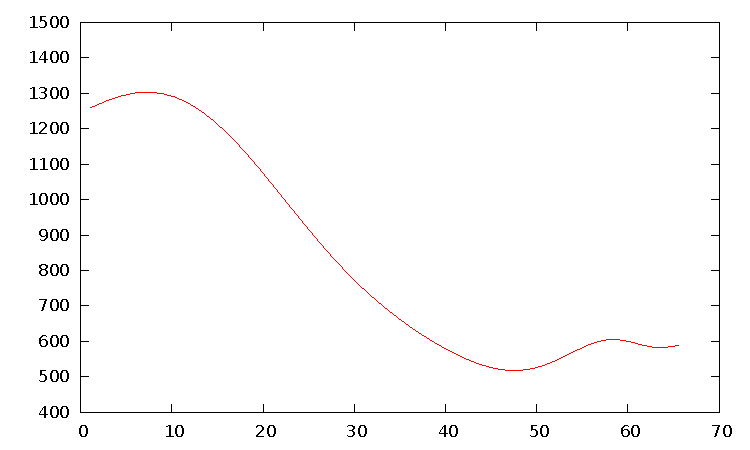
\includegraphics[scale=0.3]{middle.pdf}
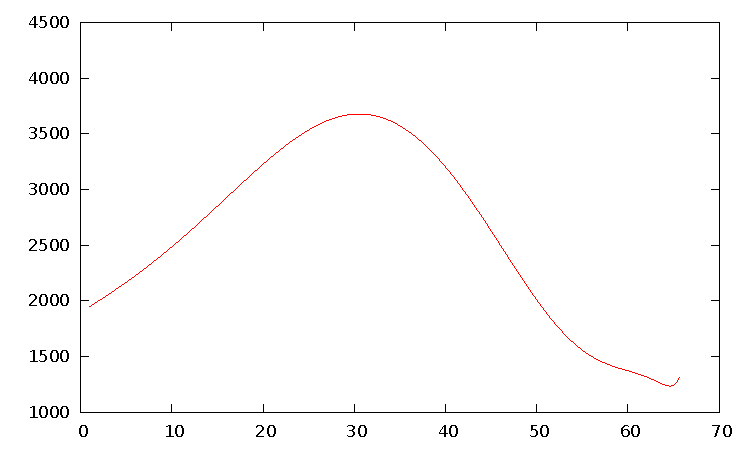
\includegraphics[scale=0.3]{far.pdf}
\caption{Proche, Milieu, Loin}
\end{figure}
\end{frame}

\begin{frame}
\frametitle{Résultats}
\begin{figure}
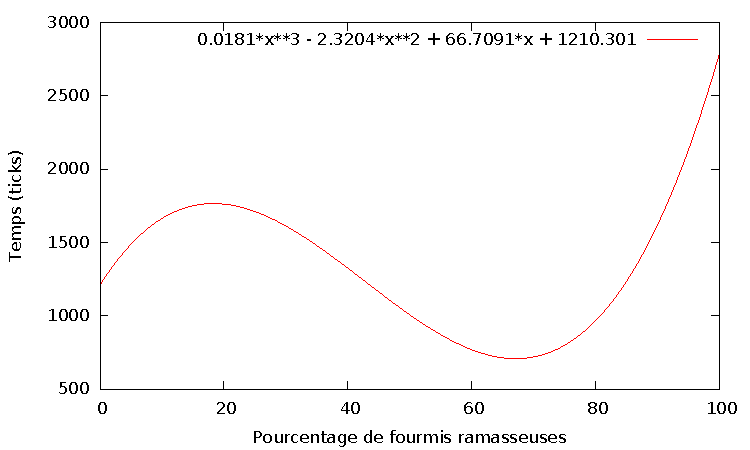
\includegraphics[scale=0.8]{avg.pdf}
\caption{Moyenne}
\end{figure}
\end{frame}

\section{Conclusion et perspectives}
\begin{frame}
\frametitle{Conclusion et Perspectives}

\begin{block}{Modèle}
\begin{math}
 f(x) = 0.0181\cdot x^3 - 2.3204\cdot x^2 + 66.7091\cdot x + 1210.3016
\end{math}
\end{block}

\begin{block}{Perspectives}
\begin{itemize}
\item comment prendre en compte le nombre de tas de nourriture ?
\item Que se passe-t-il lorsqu'il y a des nids rivaux à proximité ? D'autres types de fourmis pour défendre
\item la colonie ou se disputer les sources de nourriture ?
\end{itemize}
\end{block}
\end{frame}

\section{Credits}
\begin{frame}
\frametitle{Credits}
\begin{itemize}
\item Wilensky, U. (1997). NetLogo Ants model. \url{http://ccl.northwestern.edu/netlogo/models/Ants}. Center for Connected Learning and Computer-Based Modeling, Northwestern University, Evanston, IL.
\item Wilensky, U. (1999). NetLogo. \url{http://ccl.northwestern.edu/netlogo/}. Center for Connected Learning and Computer-Based Modeling, Northwestern University, Evanston, IL.
\end{itemize}
\end{frame}

\begin{frame}
\frametitle{Credits}
\begin{itemize}
\item Liviu A. Panait and Sean Luke. (2004). \url{http://www.cc.gatech.edu/~turk/bio_sim/articles/ant_foraging_revisited.pdf} . George Mason University, Fairfax, VA 22030.
\item Chaos–order transition in foraging behavior of ants
Lixiang Li, Haipeng Peng, Jürgen Kurths, Yixian Yang, Hans Joachim Schellnhuber
Proc Natl Acad Sci U S A. 2014 Jun 10; 111(23): 8392–8397. Published online 2014 May 27. doi: 10.1073/pnas.1407083111
\end{itemize}
\end{frame}







\end{document}






%
% %%%%% ---- THEAL
%
%\begin{frame}
%\frametitle{Introduction}
%\framesubtitle{Contexte}
%\begin{block}{ACO}
%\begin{itemize}
%\item Ant colony optimisation
%\item Travelling Salesman Problem
%\item Exploration de graphes
%\item Besoin d'étudier le comportement des fourmis
%\end{itemize}
%\end{block}
%\end{frame}
%
%\begin{frame}
%\frametitle{Introduction}
%\framesubtitle{Recherche de nourriture}
%\begin{itemize}
%\item Chercheuses et ramasseuses
%\item Chercheuses partent en éclaireur
%\item Reviennent quand elles trouvent une source de nourriture et laissent des phéromones
%\item Ramasseuses suivent la trace jusqu'à la nourriture 
%\end{itemize}
%\end{frame}
%
%\begin{frame}
%\frametitle{Problématique}
%\begin{block}{Direction des recherches}
%\begin{itemize}
%\item La présence de chercheuses a-t-elle une réelle influence sur l'efficacité de la récolte ?
%\item Si oui, quelle est cette influence ?
%\item Comment évolue-t-elle en fonction de le proportion de chercheuses ? 
%\end{itemize}
%\end{block}
%\end{frame}
%
%\begin{frame}
%\frametitle{Modélisation}
%\begin{block}{Hypothèses simplificatrices}
%\begin{itemize}
%\item Deux type de fourmis uniquement
%\item Retrouver le nid à l'instinct
%\item Pas de rivalité avec une autre colonie
%\end{itemize}
%\end{block}
%\end{frame}
%